\chapter{Encoding of processor instruction sets with explicit concurrency control}

\label{chap:PGEncoding}

The chapter is based on the results published in~\cite{cpog_encoding}. It shows how to represent processor instruction sets using CPOG formalism and provides
a ground for a concise formulation of several encoding problems, which
are reducible to the well-known Boolean satisfiability (SAT) problem
and can be efficiently solved by modern SAT solvers. Application of
all the presented techniques is demonstrated on a processor design
example.

\section{Optimal encoding of partial orders\label{sec:Optimal-encoding-problem}}

This section shows the effect of different encoding of partial orders
on the size of the resultant CPOG.

Consider a processing unit that has an accumulator register $A$ and
a general purpose register $B$, and computes four different arithmetic
functions: $(-a)$, $(a+b)$, $(a-b)$, $(-a-b)$. The event domain
contains the following events:

\renewcommand{\labelenumi}{\alph{enumi})}
\begin{enumerate}
\item Load register $A$ from memory;
\item Load register $B$ from memory;
\item Negate value stored in one of the registers;
\item Compute sum $A+B$ and store the result in $A$;
\item Save register $A$ into memory.
\end{enumerate}
The four instructions are described as partial orders of the above
events in Figure~\ref{fig-Four-DAGs-specifying} (we use \textbf{Hasse
diagrams}~\cite{1967_birkhoff_} to represent partial orders concisely,
viz. without transitive dependencies). For instance, the second instruction
(computation of $(a+b)$ shown in Figure~\ref{fig-Four-DAGs-specifying}(b))
consists of events $a$ and $b$ happening concurrently (loading of
registers $A$ and $B$), which are followed by event $d$ (addition)
and finally by event $e$ (saving the result).

\begin{figure}[h]
\begin{centering}
\subfloat[$(-a)$]{

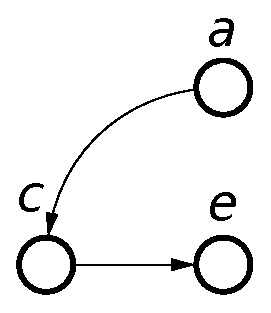
\includegraphics[scale=0.45]{fig/dag_neg}}\hfill{}\hfill{}\hfill{}\subfloat[$(a+b)$]{

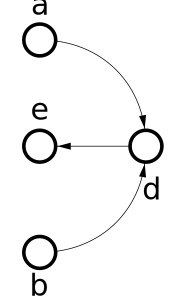
\includegraphics[scale=0.45]{fig/dag_add}}\hfill{}\hfill{}\hfill{}\subfloat[$(a-b)$]{

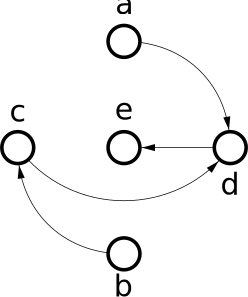
\includegraphics[scale=0.45]{fig/dag_sub}}\hfill{}\hfill{}\hfill{}\hfill{}\subfloat[$(-a-b)$]{

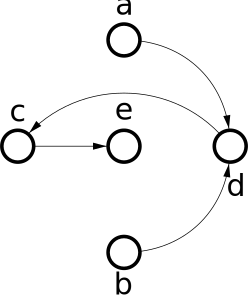
\includegraphics[scale=0.45]{fig/dag_nadd}}
\par\end{centering}

\caption{Partial orders of the instructions\label{fig-Four-DAGs-specifying}}
\end{figure}


Before synthesis of a CPOG $H=(V,\ E,\ X,\ \rho,\ \phi)$ containing
these instructions it is necessary to encode them, i.e. to derive
a set of variables $X=\{x_{1},\ x_{2},\ \dots,\ x_{m}\}$ and a set
of Boolean vectors $\{\psi_{1},\ \psi_{2},\ \dots,\ \psi_{n}\},\ \psi_{k}\in\{1,\ 0\}^{m}$
(opcodes), each of them corresponding to a particular partial order.
Note that $V$ and $E$ can be defined as unions of vertices and arcs
of the given partial orders, $\rho$ as a disjunction of generated
opcodes, and $\phi(z),\ z\in V\cup E$ as a disjunction of opcodes
corresponding to the partial orders containing $z$. Let us examine
several possible encoding schemes to see how a particular scheme affects
the resultant CPOG.

\begin{figure}[th]
\begin{centering}
\subfloat[Binary encoding (00, 01, 10, 11) and projection under opcode 01]{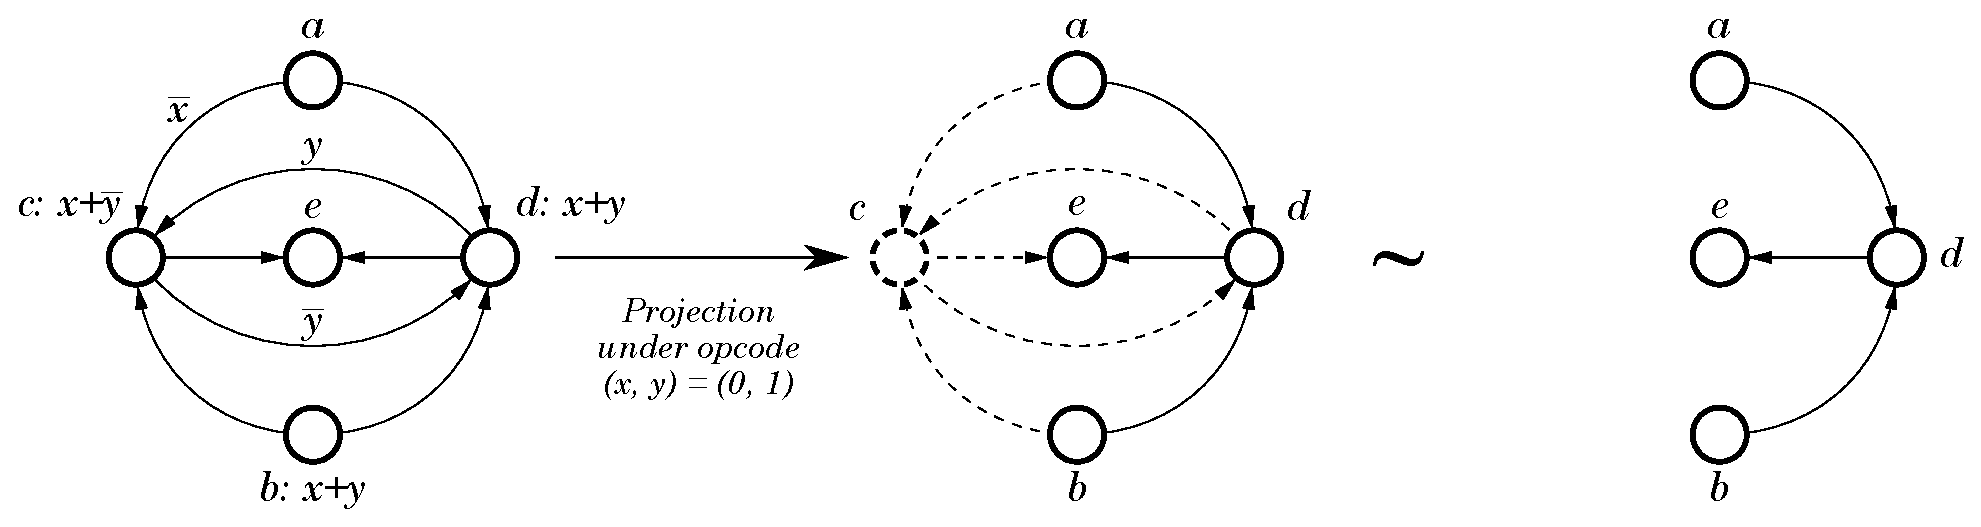
\includegraphics[scale=0.45]{fig/cpog_bin_2}}
\par\end{centering}

\begin{centering}
\subfloat[One-hot encoding (0001, 0010, 0100, 1000) and projection under opcode
0010]{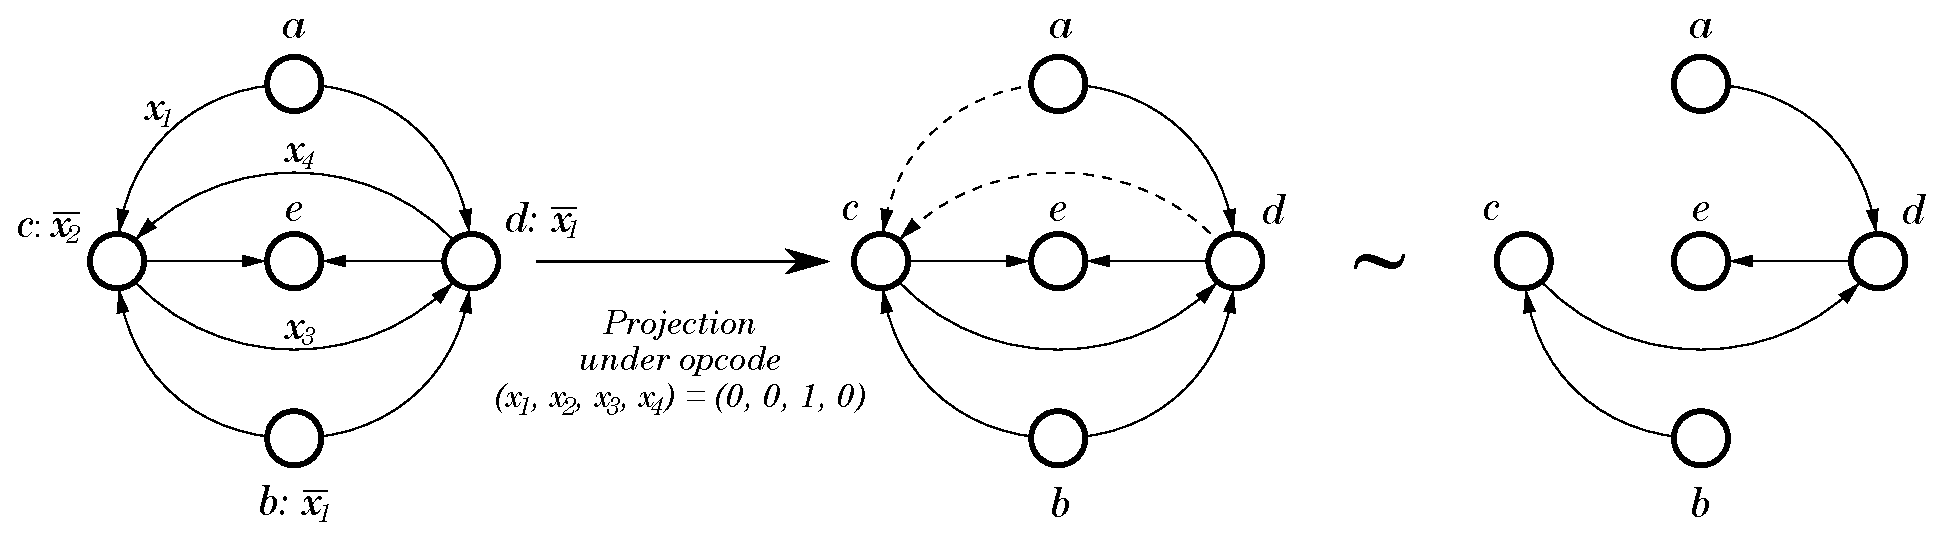
\includegraphics[scale=0.45]{fig/cpog_oh_2}}
\par\end{centering}

\centering{}\subfloat[Optimal encoding (010, 100, 111, 110) and projection under opcode
110]{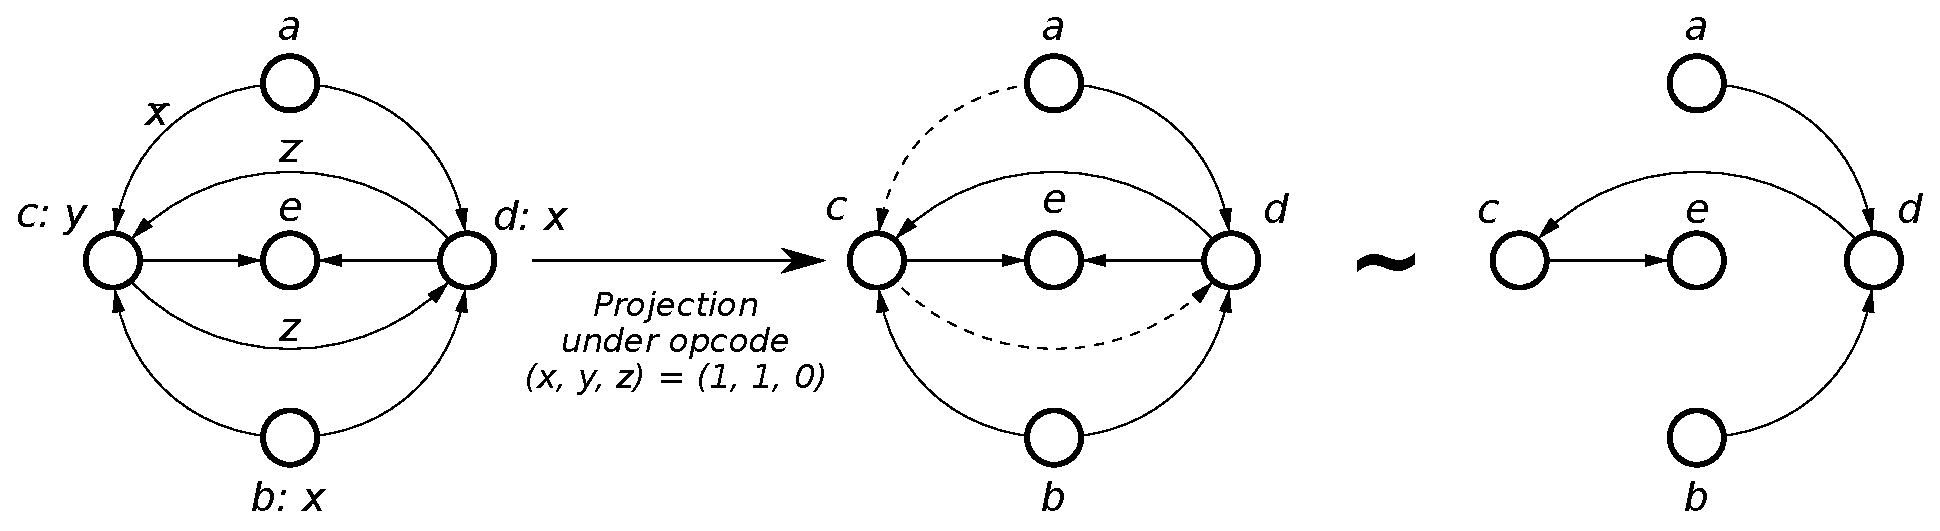
\includegraphics[scale=0.45]{fig/cpog_opt_2}}\caption{Different encoding schemes and projection examples\label{fig:Different-encoding-schemes}}
\end{figure}


\textbf{Binary encoding scheme}

This scheme uses the least possible number of variables $m=\left\lceil \log_{2}n\right\rceil $
to encode $n$ given partial orders. In our case two variables $X=\{x,\ y\}$
are used, and the opcodes are $\psi_{1}=(00)$, $\psi_{2}=(01)$,
$\psi_{3}=(10)$, and $\psi_{4}=(11)$. The synthesised CPOG and one
of its projections are shown in Figure~\ref{fig:Different-encoding-schemes}(a).
There are 9 literals in its vertex/arc conditions%
\footnote{Throughout the chapter we use operators `$+$' and `$\cdot$' to
denote Boolean disjunction (OR) and conjunction (AND), respectively.%
}.

\textbf{One-hot encoding scheme}

This is one of the most straightforward encoding schemes. It uses
$m=n$ variables to encode $n$ given partial orders such that $\psi_{k}[k]=1$
and $\psi_{k}[j]=0,\ j\neq k$. In our example, the four one-hot opcodes
are: $\psi_{1}=(1000)$, $\psi_{2}=(0100)$, $\psi_{3}=(0010)$, and
$\psi_{4}=(0001)$. Figure~\ref{fig:Different-encoding-schemes}(b)
shows the corresponding CPOG. Conditions on vertices $\{b,\ c,\ d\}$
became simpler; the total literal count was reduced to $6$. The price
for that is the increase in the number of variables from 2 to 4. Note
also that the projection under opcode $\psi_{3}=(0010)$ (shown to
the right) contains the transitive dependencies $b\rightarrow d$
and $c\rightarrow e$ which are not present in Figure~\ref{fig-Four-DAGs-specifying}(c).
Use of transitive dependencies helps to simplify arc conditions in
many cases (this and other optimisation techniques are discussed in~\cite{2010_mokhov_ieee}).

\textbf{Optimal encoding scheme}

It turns out that there is a middle-ground solution which uses the
same number of literals but only $3$ variables $X=\{x,\ y,\ z\}$.
The partial orders are encoded as $\psi_{1}=(010)$, $\psi_{2}=(100)$,
$\psi_{3}=(111)$ and $\psi_{4}=(110)$ leading to the CPOG in Figure~\ref{fig:Different-encoding-schemes}(c).
We call this encoding scheme optimal, because it is better than the
binary scheme (the resultant CPOG has fewer literals leading to a
simpler controller), and it is better than the one-hot scheme (it
uses fewer variables thus reducing the number of opcode wires coming
to the controller from the environment).

Given a CPOG $H$, there is a linear dependency between its complexity
$C(H)$, defined below, and the size of the synthesised controller~\cite{2010_mokhov_ieee}.
Figure~\ref{fig-Size-of-specification} shows a Pareto diagram comparing
different encoding schemes according to the number of variables they
use $|X|$ and complexity of the resultant CPOG. One can see that
the matrix encoding scheme~\cite{2009_mokhov_phd} produces CPOGs
with minimum possible size, but uses significantly more variables
than the binary one. We aim to reduce the number of used variables
but stay on the lower bound of CPOG complexity. In practice, the choice
of a particular encoding scheme is crucial. The resultant CPOGs (and
controllers) can differ in size by several orders of magnitude depending
on the chosen instruction codes. Now let us provide a formal definition
of CPOG optimality criteria.

\begin{figure}[h]
\begin{centering}
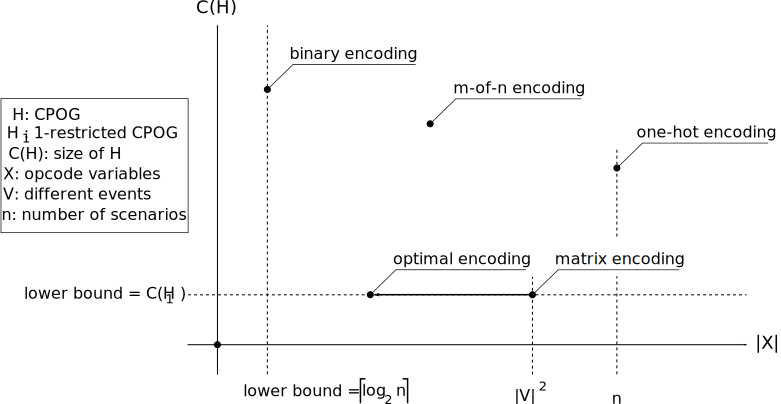
\includegraphics[width=0.75\columnwidth]{fig/encodings}

\par\end{centering}

\caption{Comparison of different encoding schemes\label{fig-Size-of-specification}}
\end{figure}

\subsection{Criteria for optimality\label{sec:Criteria-for-optimality}}

A common measure of complexity of a Boolean formula $f$ is denoted
as $C(f)$ and is defined to be the total count of literals in it~\cite{1987_wegener_book},
e.g. $C(x\cdot z+y\cdot\overline{z})=4$, $C(1)=0$, etc. Complexity
of a CPOG $H$ is measured as a sum of literals in all of its vertex
and arc conditions $\phi$, i.e.
\[
C(H)\overset{\textrm{df}}{=}\sum_{v\in V}C(\phi(v))+\sum_{e\in E}C(\phi(e))
\]
A CPOG $H=(V,\ E,\ X,\ \rho,\ \phi)$ is called $k$-\textbf{restricted}
iff its vertex and arc conditions $\phi$ are formulae having at most
$k$ literals, i.e. $\forall z\in V\cup E,\ C(\phi(z))\le k$. A \emph{$1$-}restricted
CPOG contains only formulae with single literals or constants as its
vertex and arc conditions. A $k$-restricted CPOG is called \textbf{strongly}
$k$-\textbf{restricted} iff there is a vertex or an arc with condition
having exactly $k$ literals, i.e. $\exists z\in V\cup E,\ C(\phi(z))=k$.

$C(H)$ strongly correlates with size and speed of the physical implementation
of a controller specified with $H$. Hence, we use $C(H)$ as an adequate
estimate of a CPOG $H$ efficiency. The following proposition states
that any optimal (w.r.t. measure $C$) CPOG is bound to be $1$-restricted.

\textbf{Proposition.} (Optimality) For any strongly $k$-restricted
($k>1$) CPOG $H$ there exists an equivalent%
\footnote{CPOGs are equivalent if they specify the same set of partial orders.%
} $1$-restricted CPOG $H_{1}$ such that $C(H_{1})<C(H)$.

\textbf{Proof}\textbf{\emph{.}} (Constructive). Let $n$ be the number
of partial orders contained in $H=(V,\ E,\ X,\ \rho,\ \phi)$, and
$\{\psi_{1},\ \psi_{2},\ ...,\ \psi_{n}\}$ be their encodings. It
is possible to select a $z^{+}\in V\cup E$ such that $C(\phi(z^{+}))>1$
(such $z^{+}$ must exist because $H$ is strongly restricted). 

Consider a CPOG $H'=(V,\ E,\ X\cup\{x\},\ \rho',\ \phi')$ with the
extended variable set (a variable $x$ is added), where
\[
\forall z\in V\cup E,\ \phi'(z)=\begin{cases}
\phi(z) & \text{if }z\neq z^{+}\\
x & \text{if }z=z^{+}
\end{cases}
\]
In other words, we replaced condition $\phi(z^{+})$ which had more
than one literal with condition $\phi'(z^{+})=x$ which consists of
a single literal, thus reducing the overall CPOG size by $C(\phi(z^{+}))-1>0$
literals.

New encodings $\{\psi'_{1},\ \psi'_{2},\ ...,\ \psi'_{n}\}$ are obtained
by adding an extra element $a_{k}$ (which is an assignment of $x$
in the $k$-th partial order) to the original encoding vectors%
\footnote{We use `$\circ$' to denote concatenation of Boolean vectors, e.g.
$1011\circ0=10110$.%
}: $\psi'_{k}=\psi_{k}\circ a_{k}$, where $a_{k}$ is the value of
condition $\phi(z^{+})$ under opcode $\psi_{k}$. Restriction function
$\rho$ is also modified into $\rho'$ to allow the extended opcodes.

The above procedure simplifies the original graph by relaxing one
of its conditions, without affecting any contained partial orders.
The procedure can be repeated iteratively until the resultant graph
becomes $1$-restricted (denoted as $H_{1}$). Every iteration reduces
the size by at least $1$ (because $C(\phi(z^{+}))-1>0$), which proves
the proposition.\hspace*{\fill}$\square$

Although the above proof provides a polynomial algorithm for reduction
of any CPOG to a 1-restricted form, it is rather naive in terms of
the resultant size of variable set $X$. It adds as many new variables
as there are `heavy' ($C(\phi(z^{+}))>1$) conditions in the original
graph. In the worst case it uses $|V|^{2}$ additional variables which
can be impractical. The next subsection introduces a method which
uses the least possible number of variables to encode given partial
orders into a 1-restricted CPOG.


\subsection{Method for optimal encoding\label{sec:Method-for-optimal}
}

Let $\{P_{1},\ P_{2},\ \dots,\ P_{n}\}$ be a given set of $n$ partial
orders. The objective is to synthesise a $1$-restricted CPOG $H=(V,\ E,\ X,\ \rho,\ \phi)$
and to generate opcodes $\{\psi_{1},\ \psi_{2},\ \dots,\ \psi_{n}\}$
such that $H$ contains the given partial orders and the size of variable
set $X$ is minimised.

To solve this problem it is necessary to simultaneously satisfy all
the encoding\emph{ }constraints of graph $H$.

Formally, an \textbf{encoding}\emph{ }\textbf{constraint} $\mathbf{e}(z)\in\{0,\ 1,\ -\}^{n}$
for a vertex or arc $z\in(V\cup E)$ is a vector of $n$ elements,
each corresponding to one of $n$ given partial orders. Element $\mathbf{e}(z)[k],\ 1\le k\le n$
is equal to $0$ iff condition $\phi(z)$ should evaluate to $0$
under opcode $\psi_{k}$ in order to produce correct partial order
$P_{k}$; $\mathbf{e}(z)[k]=1$ iff the condition should evaluate
to $1$; and $\mathbf{e}(z)[k]=-$ iff $\phi(z)$ can evaluate either
to $0$ or to $1$ (a \textbf{don't care} value~\cite{1994_de_micheli_book},
as explained below).

\begin{table}[h]
\begin{centering}
\begin{tabular}{|c|c|c|c|c|c|c|}
\hline 
Vertices/arcs & \multicolumn{4}{c|}{Encoding constraint $\mathbf{e}(z)$} & \multicolumn{2}{c|}{Encoding $\phi(z)$}\tabularnewline
\cline{2-7} 
\multicolumn{1}{|c|}{$z\in V\cup E$} & $(-a)$ & $(a+b)$ & $(a-b)$ & $(-a-b)$ & \multicolumn{1}{c|}{pos. only} & \multicolumn{1}{c|}{pos./neg.}\tabularnewline
\hline 
\hline 
$a,\ e$ & $1$ & $1$ & $1$ & $1$ & $1$ & $1$\tabularnewline
\hline 
$a\rightarrow d$ & $-$ & $1$ & $1$ & $1$ & $1$ & $1$\tabularnewline
\hline 
$a\rightarrow e,\ b\rightarrow e$ & $-$ & $-$ & $-$ & $-$ & $0$ & $0$\tabularnewline
\hline 
$b\rightarrow c$ & $-$ & $-$ & $1$ & $-$ & $1$ & $1$\tabularnewline
\hline 
$b\rightarrow d$ & $-$ & $1$ & $-$ & $1$ & $1$ & $1$\tabularnewline
\hline 
$c\rightarrow e$ & $1$ & $-$ & $-$ & $1$ & $1$ & $1$\tabularnewline
\hline 
$d\rightarrow e$ & $-$ & $1$ & $1$ & $-$ & $1$ & $1$\tabularnewline
\hline 
\hline 
$b,\ d$ & $0$ & $1$ & $1$ & $1$ & $x$ & $x$\tabularnewline
\hline 
$c$ & $1$ & $0$ & $1$ & $1$ & $y$ & $y$\tabularnewline
\hline 
$a\rightarrow c$ & $1$ & $-$ & $0$ & $-$ & $z$ & $\overline{x}$\tabularnewline
\hline 
$c\rightarrow d$ & $-$ & $-$ & $1$ & $0$ & $w$ & $z$\tabularnewline
\hline 
$d\rightarrow c$ & $-$ & $-$ & $0$ & $1$ & $z$ & $\overline{z}$\tabularnewline
\hline 
\end{tabular}

\par\end{centering}

\caption{Encoding constraints\label{tab:Encoding-contstraints}}
\end{table}


Table~\ref{tab:Encoding-contstraints} shows all the encoding constraints
for partial orders in Figure~\ref{fig-Four-DAGs-specifying}. For
example, vertices $a$ and $e$ appear in all the four scenarios,
so $\mathbf{e}(a)=\mathbf{e}(e)=1111$ which means that $\phi(a)=\phi(e)=1$.
On the other hand, vertices $b$ and $d$ are not present in the first
scenario, and therefore their encoding constraint is $\mathbf{e}(b)=\mathbf{e}(d)=0111$.
First 11 rows of the table contain trivial\emph{ }encoding\emph{ }constraints,
i.e. constraints which do not contain $\mathbf{e}(z)[j]=0$ and $\mathbf{e}(z)[k]=1$
simultaneously ($j\neq k$). Vertices/arcs $z\in V\cup E$ with trivial
encoding constraints can be encoded with a Boolean constant ($\phi(z)=0$
or $\phi(z)=1$, see column `Encoding' in the table). Non-trivial\emph{
}encoding\emph{ }constraints (the last 5 rows of the table) cannot
be satisfied with a constant value, and therefore we need to introduce
operational variables to encode them, e.g. it is possible to satisfy
$\mathbf{e}(b)=\mathbf{e}(d)=0111$ with variable $x$: $\phi(b)=\phi(d)=x$.

Don't care values appear in a constraint in two cases:
\begin{itemize}
\item An arc $e=(v\rightarrow u)$ is not present in a partial order together
with one of its vertices. In this case $\phi(e)$ is allowed to evaluate
not only to $0$ but also to $1$, because if one of its vertices
is excluded from the partial order ($\phi(v)=0$ or $\phi(u)=0$)
then the arc is also excluded.
\item An arc $e=(v\rightarrow u)$ is transitive (i.e. $v\rightarrow t\rightarrow u$
for some $t\in V$). Therefore $\phi(e)$ is allowed to evaluate not
only to $1$ but also to $0$ (because transitive dependency $v\rightarrow t\rightarrow u$
is enough to guarantee $v\rightarrow u$ ordering).
\end{itemize}
Encoding constraint $\mathbf{e}(a\rightarrow c)=1\!-\!0-$ combines
these two cases. The first don't care is due to exclusion of vertex
$c$ in the second scenario ($\mathbf{e}(c)=1\underline{0}11$). And
the second don't care is due to transitive dependency $a\rightarrow d\rightarrow c$
in the fourth scenario ($\mathbf{e}(a\rightarrow d)=-11\underline{1}$
and $\mathbf{e}(d\rightarrow c)=-\!-0\underline{1}$).

Two encoding constraints $\mathbf{e}_{1}$ and $\mathbf{e}_{2}$ are
\textbf{conflicting} iff
\[
\exists_{1\le k\le n},\ (\mathbf{e}_{1}[k]=1\wedge\mathbf{e}_{2}[k]=0)\vee(\mathbf{e}_{1}[k]=0\wedge\mathbf{e}_{2}[k]=1)
\]
In other words, it is impossible to find a Boolean vector satisfying
both constraints. For example, $\mathbf{e}(a\rightarrow c)=1\!-\!0-$
and $\mathbf{e}(c\rightarrow d)=-\!-\!10$ are conflicting, because
$\mathbf{e}(a\rightarrow c)[3]=0$ and $\mathbf{e}(c\rightarrow d)[3]=1$.
On the other hand, $\mathbf{e}(a\rightarrow c)=1\!-\!0-$ and $\mathbf{e}(d\rightarrow c)=-\!-\!01$
are not conflicting since vector $1001$ satisfies both of them. It
means that they can be resolved with the same variable (variable $z$
in Table~\ref{tab:Encoding-contstraints}, see column `Encoding:
pos. only').

The optimal encoding problem can now be formulated in terms of conflicting
encoding constraints: find an assignment of variables $\{x_{1},\ x_{2},\ \dots,\ x_{m}\}$
to constraints such that all pairs of the conflicting constraints
are assigned different variables and $m$ is minimised~\cite{2009_mokhov_phd}.
This problem belongs to the NP-complete complexity class and can be
reduced to the graph vertex colouring problem~\cite{2001_cormen_mit}:
a constraint must be `coloured' with a variable $x_{k}$ and any
two conflicting constraints must have different colours~\cite{2009_mokhov_phd}.

Figure~\ref{fig:Conflict-graph-colouring}(a) shows the conflict
graph for non-trivial encoding constraints from Table~\ref{tab:Encoding-contstraints}
and one of its optimal vertex colourings. It uses 4 `colours' $X=\{w,\ x,\ y,\ z\}$
and establishes the following encoding: $\psi_{1}=(0011)$, $\psi_{2}=(0100)$,
$\psi_{3}=(1110)$, and $\psi_{4}=(0111)$. This colouring is also
given in column `Encoding: pos. only' of the table. The synthesised
CPOG is shown in Figure~\ref{fig:Conflict-graph-colouring}(c); it
has the same size as the one-hot solution shown before but contains
only positive literals in its vertex/arc conditions.

Note that although encoding constraints $\mathbf{e}(c\rightarrow d)=-\!-\!01$
and $\mathbf{e}(d\rightarrow c)=-\!-\!10$ are conflicting they complement
each other. This opens another optimisation opportunity: it is possible
to resolve both constraints with a single variable $x$ using conditions
with complementary literals $x$ and $\overline{x}$, thus potentially
halving the number of used variables. In order to exploit this, we
build an \textbf{extended conflict graph} which contains two vertices
for every encoding constraint $\mathbf{e}(z)$: one for the original
constraint and one for its inversion $\overline{\mathbf{e}}(z)$ which
is defined as
\[
\forall1\le k\le n,\ \overline{\mathbf{e}}(z)[k]=\begin{cases}
0 & \text{if }\mathbf{e}(z)[k]=1\\
1 & \text{if }\mathbf{e}(z)[k]=0\\
- & \text{if }\mathbf{e}(z)[k]=-
\end{cases}
\]
Exactly one vertex of every pair $\{\mathbf{e}(z),\ \overline{\mathbf{e}}(z)\}$
has to be coloured. If the vertex corresponding to an inverted constraint
$\overline{\mathbf{e}}(z)$ is chosen to be coloured with variable
$x$ it means that the constraint is resolved with negative condition
$\phi(z)=\overline{x}$. See Figure~\ref{fig:Conflict-graph-colouring}(b)
for the extended conflict graph of the example problem and its optimal
colouring. This colouring can also be found in column `Encoding:
pos./neg.' of Table~\ref{tab:Encoding-contstraints}. The synthesised
CPOG is shown in Figure~\ref{fig:Conflict-graph-colouring}(d) and
the generated opcodes of partial orders are $\psi_{1}=(010)$, $\psi_{2}=(100)$,
$\psi_{3}=(111)$ and $\psi_{4}=(110)$. This solution uses both positive
and negative literals for resolution of conflicting encoding constraints,
e.g. $\phi(c\rightarrow d)=z$ and $\phi(d\rightarrow c)=\overline{z}$,
resulting in only three operational variables $X=\{x,\ y,\ z\}$.
It is the optimal CPOG specification of the four partial orders from
Figure~\ref{fig-Four-DAGs-specifying}, there is no solution which
uses fewer literals.

The vertex colouring problem can be converted into an instance of
the Boolean satisfiability problem (SAT) for efficient solution as
explained in Section~\ref{sec:SAT-formulation}.

\begin{figure}[h]
\begin{centering}
\hfill{}\subfloat[Colouring with positive literals only]{\begin{centering}
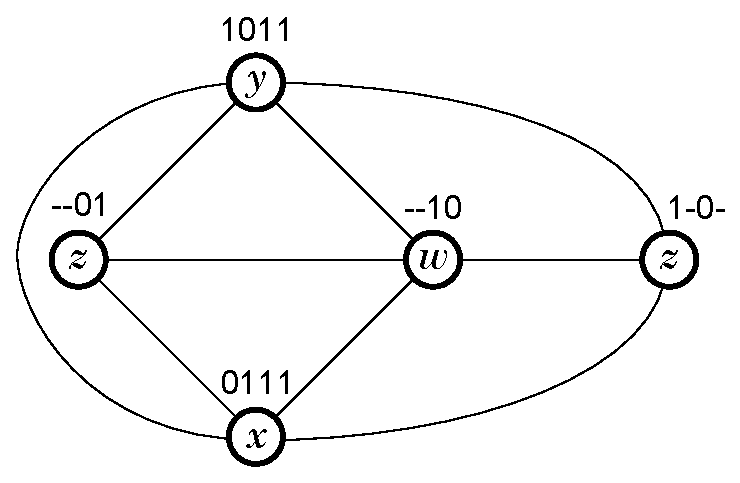
\includegraphics[bb=0bp 0bp 425bp 270bp,scale=0.45]{fig/conflict_graph_col}
\par\end{centering}

}\hfill{}\subfloat[Colouring with positive and negative literals]{\centering{}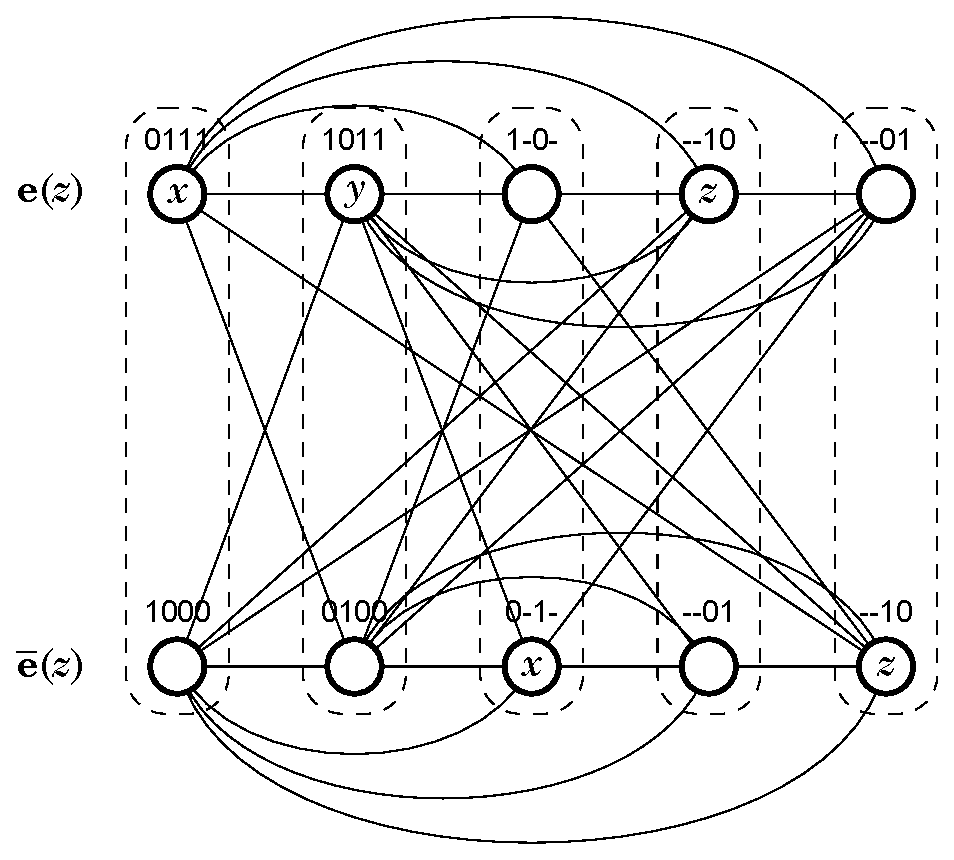
\includegraphics[scale=0.45]{fig/conflict_graph_inv}}\hfill{}
\par\end{centering}

\begin{centering}
\hfill{}\subfloat[CPOG with positive literals]{

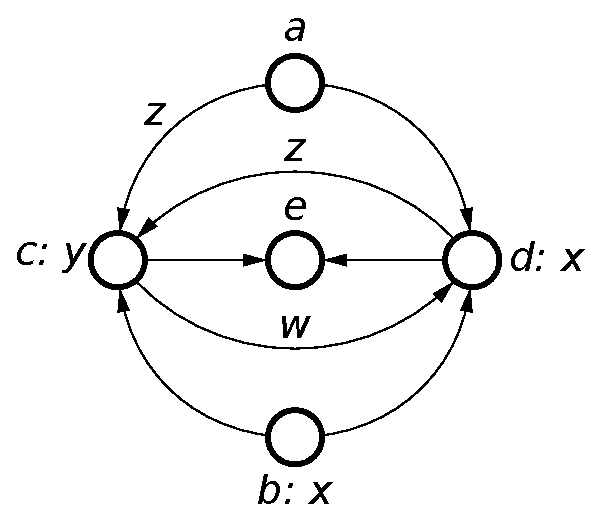
\includegraphics[scale=0.45]{fig/cpog_opt_woinv}}\hfill{}\subfloat[CPOG with positive and negative literals]{

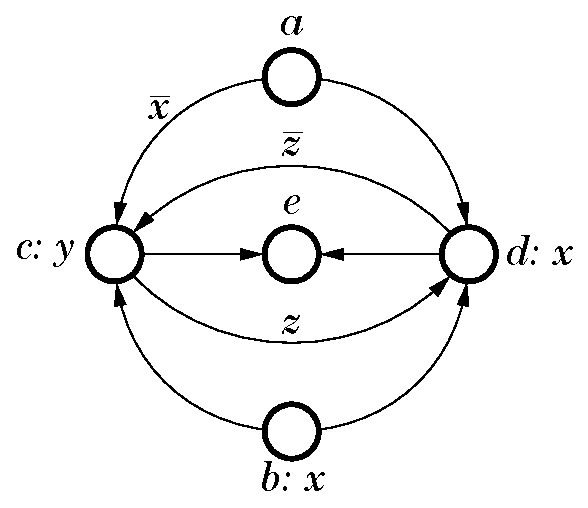
\includegraphics[scale=0.45]{fig/cpog_opt_w_inv}}\hfill{}
\par\end{centering}

\caption{Conflict graphs colouring and corresponding synthesised CPOGs\label{fig:Conflict-graph-colouring}}
\end{figure}



\subsection{Generating optimal opcodes of specified length\label{Sec:Generating-optimal-opcodes}}

The optimal encoding method presented above generates the smallest
CPOG description of a set of partial orders but the number of used
variables cannot be controlled; in many practical cases it will use
more variables than is affordable under the design or technology constraints.
In this section we briefly describe a method for generating the smallest
CPOG given a limit on the number of variables, i.e. given the required
length of the instruction codes.

Let $L$ be the given limit on the number of variables. The method
is based on the same principle as before: we generate all non-trivial
encoding constraints and try to satisfy them with opcode variables.
Only $L$ of them are free variables $X=\{x_{1},\ x_{2},\ ...,\ x_{L}\}$;
other variables $F=\{f_{1},\ f_{2},\ ...,\ f_{m}$\} are not free
--- they are expressed in terms of variables from $X\cup F$ using
Boolean binary functions, e.g. $f_{1}=x_{1}+\overline{x_{3}}$, $f_{2}=f_{1}\cdot x_{2}$,
etc. As $L$ is fixed all we have to do is to minimise the number
of non-free variables $m$. This minimisation problem requires exploration
of large search space; fortunately, it still belongs to the NP complexity
class and we can reduce it to the SAT problem: the solver has to `guess'
all the opcodes, formulae of variables in $F$, and allocation of
all variables $X\cup F$ to the non-trivial encoding constraints.
See the next section for implementation details.

We used a processor design example as our benchmark to validate all
the instruction code synthesis techniques presented in this section.
The results are discussed in Section~\ref{sec-processor}.



\section{SAT formulation\label{sec:SAT-formulation}}

This section presents SAT formulations of the optimal encoding problems
described in the previous section.

The Boolean satisfiability problem (SAT) is to decide whether a given
Boolean formula $F(x_{1},\ x_{2},\ \dots,\ x_{n})$ is satisfiable
or not, i.e. if it is possible to find an assignment of Boolean values
$(\alpha_{1},\ \alpha_{2},\ \dots,\ \alpha_{n})\in\{0,\ 1\}^{n}$
to the variables $(x_{1},\ x_{2},\ \dots,\ x_{n})$ which makes the
formula true: $F(\alpha_{1},\ \alpha_{2},\ \dots,\ \alpha_{n})=1$.
As SAT is a decision (not optimisation) problem, we define a cost
function and use a binary search to minimise its value by calling
the SAT solver with different cost constraints.

We have implemented all the techniques presented in this section in
an automated software tool which uses \noun{MiniSAT}~\cite{2004_miniSAT_lncs}
as a SAT solver engine. \noun{MiniSAT} operates on CNF (conjunctive
normal form) representations of Boolean formulae. Since our SAT-instances
are not necessarily given in CNF, we implemented their automated conversion
to CNF formulae. This conversion introduces intermediate variables
but the overall size of the obtained formula is linear with respect
to the size of the given SAT-instance.



\subsection{Optimal encoding with unconstrained code length}

To solve the unconstrained optimal encoding problem described in Subsection~\ref{sec:Method-for-optimal}
we minimise the number of colours used for a conflict graph colouring.
Minimisation is performed by solving a series of instances of the
following decision problem.

Let $G=(V,\ E)$ be an extended conflict graph, where vertices $V$
correspond to encoding constraints and edges $E\subseteq V\times V$
to conflicts between them. $V$ contains both original $V_{o}=\{\mathbf{e}_{1},\ \mathbf{e}_{2},\ \dots,\ \mathbf{e}_{n}\}$
and inverted $V_{i}=\{\mathbf{\overline{\mathbf{e}}}_{1},\ \mathbf{\overline{\mathbf{e}}}_{2},\ \dots,\ \mathbf{\overline{\mathbf{e}}}_{n}\}$
constraints, such that $V=V_{o}\cup V_{i}$. The problem is to find
a colouring of $G$ which uses no more than $m$ colours.

For every pair of vertices $(\mathbf{e}_{k},\ \mathbf{\overline{\mathbf{e}}}_{k})$
we introduce a Boolean variable $p_{k}$ and an integer number $c_{k}$
whose values have to be found by the SAT solver: $p_{k}$ indicates
which of the two vertices is coloured -- if $p_{k}=1$ (resp. $p_{k}=0$)
then $\mathbf{e}_{k}$ (resp. $\overline{\mathbf{e}}_{k}$) is coloured,
while $c_{k}$ represents the colour of the chosen vertex. 

The SAT problem $\mathcal{ENCODE}$ consists of four constraints:
\[
\mathcal{ENCODE}=\mathcal{NUM}\cdot\mathcal{COL}_{oo}\cdot\mathcal{COL}_{oi}\cdot\mathcal{COL}_{ii}
\]
where $\mathcal{NUM}$ restricts colours such that $0\le c_{k}<m$.
Encoding of numbers $c_{k}$ in Boolean domain can be different, for
example, if we use binary encoding we need $\left\lceil \log_{2}m\right\rceil $
bits for each $c_{k}$. Implementation of $\mathcal{NUM}$ depends
on the chosen encoding; its general form is:
\[
\mathcal{NUM}=\prod_{1\le k\le n}(0\le c_{k})\cdot(c_{k}<m)
\]
Constraints $\mathcal{COL}$ check that adjacent vertices are assigned
different colours:
\[
\mathcal{COL}_{oo}=\prod_{(\mathbf{e}_{j},\ \mathbf{e}_{k})\in E\cap(V_{o}\times V_{o})}(p_{j}\cdot p_{k})\Rightarrow(c_{j}\neq c_{k})
\]
\[
\mathcal{COL}_{oi}=\prod_{(\mathbf{e}_{j},\ \overline{\mathbf{e}}_{k})\in E\cap(V_{o}\times V_{i})}(p_{j}\cdot\overline{p_{k}})\Rightarrow(c_{j}\neq c_{k})
\]
\[
\mathcal{COL}_{ii}=\prod_{(\overline{\mathbf{e}}_{j},\ \overline{\mathbf{e}}_{k})\in E\cap(V_{i}\times V_{i})}(\overline{p_{j}}\cdot\overline{p_{k}})\Rightarrow(c_{j}\neq c_{k})
\]
If we assume that complexity of comparison operations over numbers
$c_{k}$ is $C$, then the overall complexity of $\mathcal{ENCODE}$
is $\Theta((|V|+|E|)\cdot C)$. In particular, in case of binary encodings%
\footnote{Formula $(a<b)$ for binary numbers comparison is $(a<b)=\overline{a_{0}}\cdot b_{0}+(a_{0}=b_{0})\cdot(a'<b')$
where $a'$ and $b'$ are obtained from $a$ and $b$ by removal of
their most significant digits ($a_{0}$ and $b_{0}$); the formula
is linear with respect to the lengths of $a$ and $b$.%
} the complexity is $\Theta((|V|+|E|)\cdot\log m)$. Depending on the
chosen number encodings, there are from $\Theta(|V|\cdot\log m)$
to $\Theta(|V|\cdot m)$ free variables.

If $L$ is the minimum value of $m$ for which formula $\mathcal{ENCODE}$
is satisfiable then the optimal encoding uses $L$ variables $X=\{x_{1},\ x_{2},\ ...,\ x_{L}\}$.
Values $p_{k}$ and $c_{k}$ which satisfy the formula are used to
resolve encoding constraints $\mathbf{e}_{k}$ in the following way:
if $p_{k}=1$ then $\mathbf{e}_{k}$ is resolved by $x_{c_{k}}$,
otherwise it is resolved by $\overline{x_{c_{k}}}$.


\subsection{Optimal encoding with constrained code length}

The constrained version of the optimal encoding problem (see Subsection~\ref{Sec:Generating-optimal-opcodes})
is significantly more complicated and computationally intensive. It
requires finding a set of Boolean functions of $L$ arguments (where
$L$ is the specified code length) and there are $2^{2^{L}}$ of them
-- it is impossible to explore search spaces of such magnitudes, e.g.
$2^{2^{8}}$ roughly equals to the number of atoms in the universe.
To cope with this, we reduce the search space to 2-argument Boolean
functions only. From the practical point of view this is justified
by the fact that most modern technology libraries contain only 2-
or 3-input logic gates anyway. Importantly, every complex function
can be represented as a composition of simpler ones, therefore our
approach can find any function, albeit at the cost of introducing
intermediate variables. This is similar to what actually happens during
technology mapping\emph{ }and\emph{ }logic decomposition\emph{ }of
functional components into hardware gates~\cite{2002_cortadella_book}\cite{1994_de_micheli_book}.

Formally, let $(\mathbf{e}_{1},\ \mathbf{e}_{2},\ \dots,\ \mathbf{e}_{n})$
be a set of encoding constraints defined in Subsection~\ref{sec:Method-for-optimal},
$S$ be the number of scenarios, and $L$ be the required code length.
We are looking for such a vector $(\psi_{1},\ \psi_{2},\ \dots,\ \psi_{S})$
of $L$-bit encodings and $n$ functions $F_{j},\ 1\le j\le n$ such
that $F_{j}(\psi_{k})=\mathbf{e}_{j}[k]$ for every scenario $1\le k\le S$
(unless $\mathbf{e}_{j}[k]$ is a don't care value).

We represent a set of functions $F$ as a combinational circuit consisting
of $G$ 2-input Boolean gates, where $G$ is the value to be minimised.
An output of the circuit can be taken directly from one of its inputs
or be produced by a gate. In addition, any output can be inverted:
\[
F_{j}(\psi)=\mathit{select}(Signals(\psi),\ \mathit{oSelector}_{j})\oplus\mathit{Inv}_{j}
\]


Here $Signals(\psi)$ is a function computing all circuit signals
including both circuit inputs (given by parameter $\psi$) and gate
outputs, $\mathit{oSelector}_{j}$ is the number indicating which
circuit signal is `connected' to the $j$-th circuit output, function
$\mathit{select(V,\ k)}$ selects $k$-th element from a given vector
$V$, and $Inv_{j}=1$ iff $j$-th circuit output is inverted. Implementation
of function $select(V,\ k)$ depends on the encoding of $k$ (we used
one-hot encoding in this case, which allows for simpler implementation).
Circuit signals are computed as follows:
\[
\begin{cases}
\mathit{Signals}(\psi) & =\mathit{Wires}_{G}(\psi)\\
\mathit{Wires}_{k}(\psi) & =\begin{cases}
\psi & \textrm{\,\,\ if}\, k=0\\
\mathit{Wires}_{k-1}(\psi)\circ\mathit{Gate}_{k}(\psi) & \textrm{\,\,\ if}\,0<k\le G
\end{cases}\\
\mathit{Gate}_{k}(\psi) & =\mathit{arg}_{1,k}(\psi)\cdot\mathit{arg}_{2,k}(\psi)\\
\mathit{arg}_{j,k}(\psi) & =select(\mathit{Wires}_{k-1}(\psi),\ \mathit{aSelector}_{j,k})\oplus\mathit{InvArg}_{j,k}
\end{cases}
\]
In other words, a set of wires is initially equal to the set of circuit
inputs $(\mathit{Wires}_{0}(\psi)=\psi)$ and then is iteratively
extended by appending $Gate_{k}$ to the previously computed set of
wires $Wires_{k-1}$. Eventually, after $G$ iterations we obtain
the set of all signals $\mathit{Signals}(\psi)=\mathit{Wires}_{G}(\psi)$.
Every $Gate_{k}$ corresponds to an AND gate with possible input inversions
(indicated by $\mathit{InvArg}_{0,k}$ and $\mathit{InvArg}_{1,k}$).
Its arguments are selected by $\mathit{aSelector}_{0,k}$ and $\mathit{aSelector}_{1,k}$
from the set of wires computed in the previous iteration. This guarantees
the absence of combinational loops.

As every signal in the circuit can be optionally inverted (by setting
$\mathit{Inv}_{j}=1$ or $\mathit{InvArg}_{j,k}=1$), the resultant
gate basis includes 8 logic gates: AND, OR, NAND, NOR, plus 4 other
gates, obtained from these by inversion of exactly one of their inputs
(they do not have commonly adopted names, apart, perhaps, from Boolean
implication $x\Rightarrow y$ which corresponds to OR($\overline{x}$,
$y$)). We have also investigated a simpler basis, consisting of only
NAND gates with no optional input inversions. The basis leads to smaller
search space and works faster, but, as expected, produces larger circuits
(see Figure~\ref{fig:Comparison-of-different} for a comparison of
two bases on a processor example). If the NAND basis is used then
free variables $\mathit{InvArg}_{j,k}$ can be dropped and the formulae
for $\mathit{Gate}_{k}(\psi)$ and $\mathit{arg}_{j,k}(\psi)$ should
be modified as follows: 
\[
\begin{cases}
\mathit{Gate}_{k}(\psi) & =\overline{\mathit{arg}_{1,k}(\psi)\cdot\mathit{arg}_{2,k}(\psi)}\\
\mathit{arg}_{j,k}(\psi) & =select(\mathit{Wires}_{k-1}(\psi),\ \mathit{aSelector}_{j,k})
\end{cases}
\]
We tried to extend the 8-gate basis by addition of gates XOR and XNOR
but on practical examples it did not bring any benefit in terms of
the number of used gates, while significantly increasing the computation
time (due to additional free variables $\mathit{IsXor_{k}}$ and more
complex $\mathit{Gate}_{k}(\psi)$ functions).

In case of the standard 8-gate basis the SAT solver has to assign
the following free variables: $\psi_{j}[k]$ ($1\le j\le S,\ 1\le k\le L$),
$Inv_{j}$ ($1\le j\le n$), $\mathit{InvArg}_{0,j}$ and $\mathit{InvArg}_{1,j}$
($1\le j\le G$). Also it has to find numbers $\mathit{oSelector}_{j}$
($1\le j\le n$), $\mathit{aSelector}_{0,j}$ and $\mathit{aSelector}_{1,j}$
($1\le j\le G$). All other variables are derived.

The SAT problem $\mathcal{ENCODE}$ consists of two constraints:
\[
\mathcal{ENCODE}=\mathcal{NUM}\cdot\mathcal{EVAL}
\]
 Constraint $\mathcal{NUM}$ restricts all the selectors to their
domains:
\[
\mathcal{NUM}=\prod_{1\le j\le n}(1\le\mathit{oSelector}_{j})\cdot(\mathit{oSelector}_{j}\le L+G)\cdot\prod_{{1\le j\le2\atop 1\le k\le G}}(1\le\mathit{aSelector}_{j,k})\cdot(\mathit{aSelector}_{j,k}<L+k)
\]
Constraint $\mathcal{EVAL}$ checks that the circuit outputs satisfy
the encoding constraints:
\[
\prod_{{1\le j\le n\atop 1\le k\le S}}(\mathbf{e}_{j}[k]\neq-)\Rightarrow(F_{j}(\psi_{k})\Leftrightarrow\mathbf{e}_{j}[k])
\]


If $G_{min}$ is the minimum value of $G$ for which formula $\mathcal{ENCODE}$
is satisfiable then the optimal encoding is obtained in vectors $\psi_{j}$
($1\le j\le S$), an encoding constraint $\mathbf{e}_{k}$ is resolved
by function $F_{j}(\psi)$, and the circuit which produces these functions
contains $G_{min}$ gates.

We tried binary and one-hot number encodings in our implementation.
In both cases the complexity of the formula is $\Theta(S\cdot G\cdot(G+L))$.
The number of free variables is $\Theta(S\cdot L+(G+n)\cdot C)$,
where $C$ is $\log(G+L)$ and $G+L$ for binary and one-hot encodings,
respectively. In practice, one-hot encoding proved to be more efficient
despite significantly larger number of free variables. This can be
explained by the fact that one-hot encoding leads to simpler constraints.


\subsection{Support for dynamic variables\label{sub:Support-for-dynamic}}

A lot of practical applications require the use of \textbf{dynamic
variables}, i.e. such variables that can change their values during
execution of a partial order and affect its further execution flow~\cite{2009_mokhov_phd}.
An example of such application, a processor microcontroller, is discussed
in the next section.

Dynamic variables manifest themselves as encoding constraints with
non-constant elements, e.g. $\mathbf{e}=110y1\overline{y}$, which
means that in the fourth scenario the corresponding condition has
to evaluate to some dynamic variable $y$ and in the sixth scenario
it has to evaluate to $\overline{y}$. To compute the optimal encoding
with such non-constant constraints we have to modify the method from
the previous subsection in the following way.

Let $y$ be a dynamic variable. We generate formula $\mathcal{ENCODE}_{0}$
(resp. $\mathcal{ENCODE}_{1}$) using encoding constraints where $y$
is replaced by 0 (resp. 1). Note that the free variables in both formulae
have to be the same and we have to add $y$ into the set of circuit
inputs. Then we use the SAT solver to find an assignment that satisfies
$\mathcal{ENCODE}_{0}\cdot\mathcal{ENCODE}_{1}$. Interpretation of
the resulting assignment is the same apart from the added input signal
$y$. In case of more than one dynamic variable, the process should
be repeated for each of them. Potentially this leads to an exponential
explosion of the formula. Fortunately, the number of dynamic variables
is rather small in practice, thus the explosion is not dramatic.

It is still possible to avoid the explosion of the formula by conversion
of the problem into an instance of 2-QBF problem (a quantified Boolean
formula with two quantifiers~\cite{2004_ranjan_qbf}):
\[
\exists X\,\forall Y\ \mathcal{ENCODE}
\]
where $X$ represents the set of all free variables, and $Y$ stands
for the set of dynamic variables. However, conversion of a formula
into 2-QBF does not necessarily reduce the computation time needed
to find its satisfying assignment. Implementation of a tool based
on a 2-QBF solver is a subject of future work.

The next section demonstrates application of this technique in a processor
microcontroller design.


\section{Processor design example\label{sec-processor}
}

This section demonstrates application of the CPOG-based methodology
to specification and synthesis of processor microcontrollers, and
discusses the results of optimal instruction encoding methods presented
in the previous section. Specification of such a complex system as
a processor starts at the architectural level which helps to deal
with the system complexity by structural abstraction~\cite{1994_de_micheli_book}.
Numerous processor architectures have emerged since fundamental von
Neumann architecture\emph{~}\cite{1946_burks_architecture} and Harvard
architecture\emph{~}\cite{1946_aiken_calculator} were proposed.
The example processor is built on the basis of Harvard architecture;
however, the method for optimal encoding of instructions presented
here is applicable to both architectures, including their
numerous derivatives.

\begin{figure}
\begin{centering}
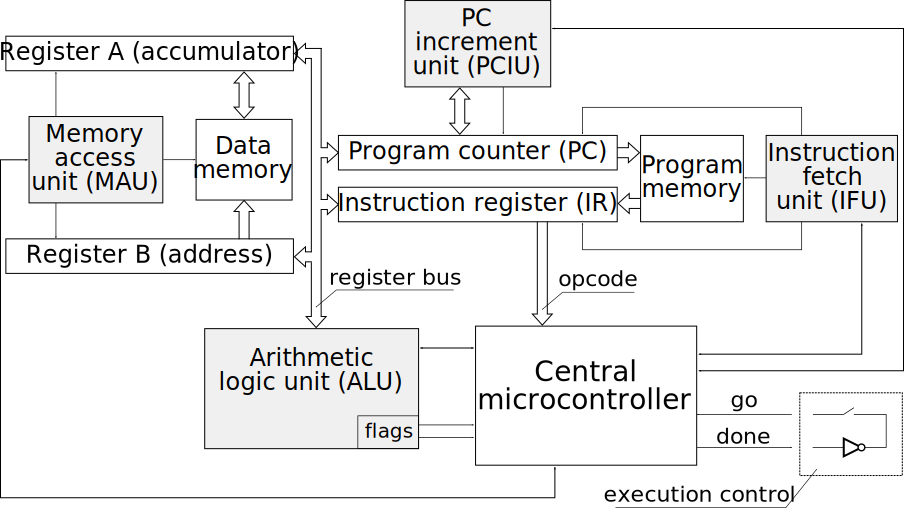
\includegraphics[width=0.75\columnwidth]{fig/processor_architecture}

\par\end{centering}

\caption{Architecture of example processor\label{app-fig-Architecture-of-example}}
\end{figure}



\subsection{Architecture}

Figure~\ref{app-fig-Architecture-of-example} shows the architecture
of the example processor. Separate \textbf{Program memory} and \textbf{Data
memory} blocks are accessed via \textbf{Instruction fetch} (IFU) and
\textbf{Memory access} (MAU) operational units, respectively. The
other two operational units are: ALU and \textbf{Program counter increment
unit} (PCIU). The units are controlled via request-acknowledgement
interfaces (depicted as bidirectional arrows) by \textbf{Central microcontroller}
which is our primary specification and synthesis objective. 

There are four registers: general purpose registers $A$ and $B$,
\textbf{Program counter} (PC) which stores address of the current
instruction in the program memory, and \textbf{Instruction register}
(IR) which stores opcode of the current instruction. For the purpose
of this example the actual width of the registers (the number of bits
they can store) is not important. ALU has access to all the registers
via the register bus; MAU accesses only general purpose registers;
IFU reads opcode of the next instruction into IR given its address
in PC; PCIU is responsible for incrementing PC (moving to the next
instruction). The microcontroller has access to the opcode and ALU
\textbf{flags} (information about the current state of ALU which is
used in branching instructions).


\subsection{Design of instruction set\label{app-sub-Design-of-instruction}}

Now we have to define the set of instructions of the processor. Rather
than to list every single instruction it is easier to describe classes
of instructions with the same \textbf{addressing mode}~\cite{mspmanual}
and partial order representation.

\textbf{ALU operation Rn to Rn}

An instruction from this class takes two operands stored in general
purpose registers $\{A,\ B\}$, performs an operation over them, and
writes the result back into one of them (so called \textbf{register
direct addressing mode}). Examples: $\mathit{ADD\ A,\ B}$ -- addition
$A=A+B$; $\mathit{MOV\ B,\ A}$ -- assignment $B=A$. Figure~\ref{app-fig-Scenarios-of-8}(a)
shows the corresponding partial order of actions that have to be performed:
ALU works concurrently with PC increment (PCIU) and the next instruction
fetch (IFU) actions. As soon as both concurrent branches are completed,
the processor is ready to execute the next instruction. Note that
it is not important for the microcontroller which particular ALU operation
is being executed ($\mathit{ADD}$, $\mathit{MOV}$, or any other)
because the partial order of actions is not affected by this choice.
It is responsibility of ALU to detect which operation it has to perform
according to the current opcode. Therefore, it is sufficient to specify
only 8 behavioural scenarios of the microcontroller (as there are
8 classes of instructions).

\begin{figure}
\begin{centering}
\subfloat[ALU op. Rn to Rn]{

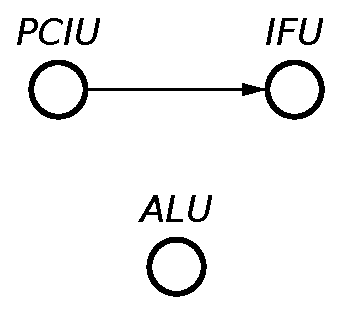
\includegraphics[scale=0.36]{fig/po_ALU_Rn_Rn}}\hfill{}\subfloat[ALU op. \#123 to Rn]{

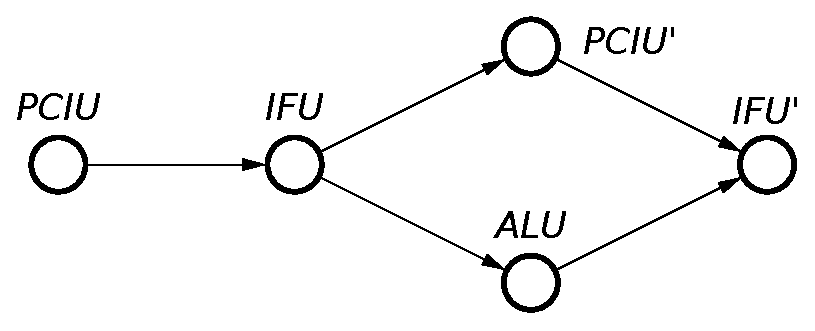
\includegraphics[scale=0.36]{fig/po_ALU_123_Rn}}\hfill{}\subfloat[ALU op. Rn to PC]{

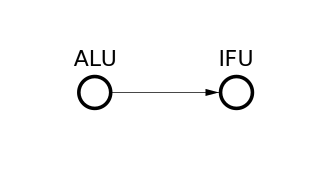
\includegraphics[scale=0.36]{fig/po_ALU_Rn_PC}}\hfill{}\subfloat[ALU op. \#123 to PC]{

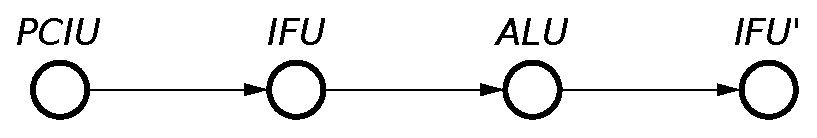
\includegraphics[scale=0.36]{fig/po_ALU_123_PC}}
\par\end{centering}

\begin{centering}
\subfloat[Memory access]{

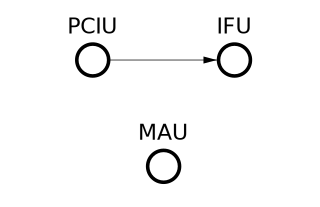
\includegraphics[scale=0.36]{fig/po_MAU}}\hfill{}\subfloat[Cond. ALU op. Rn to Rn]{

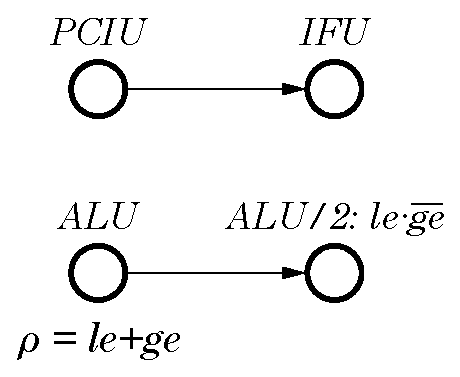
\includegraphics[scale=0.36]{fig/po_CALU_Rn_Rn}}\hfill{}\subfloat[Cond. ALU op. \#123 to Rn]{

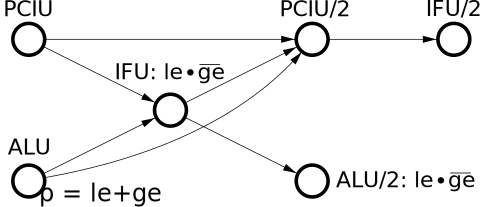
\includegraphics[scale=0.36]{fig/po_CALU_123_Rn}}\hfill{}\subfloat[Cond. ALU op. \#123 to PC]{

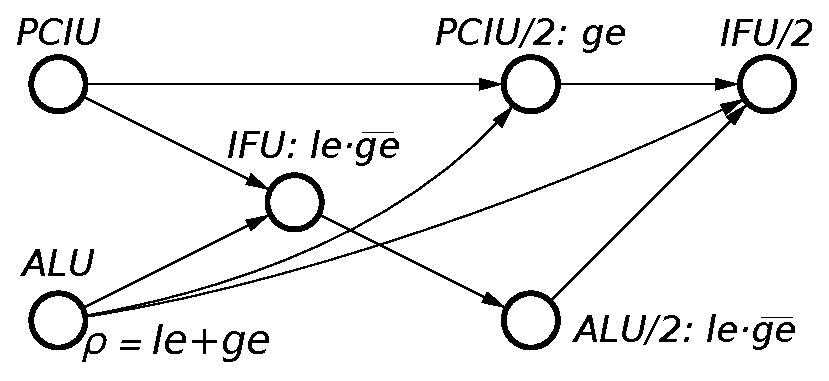
\includegraphics[scale=0.36]{fig/po_CALU_123_PC}}
\par\end{centering}

\caption{Conditional partial order specifications of 8 instruction classes\label{app-fig-Scenarios-of-8}}
\end{figure}


\textbf{ALU operation \#123 to Rn}

In this set of instructions one of the operands is register and another
is a constant which is given immediately after the instruction opcode
(e.g. $\mathit{SUB\ A,\ \#1}$ -- decrement $A$ by one), hence the
name: \textbf{immediate addressing mode}. Figure~\ref{app-fig-Scenarios-of-8}(b)
shows the partial order of actions for such an instruction. At first,
the constant has to be fetched into IR (events PCIU and IFU). Then
ALU is executed concurrently with another increment of PC. Finally,
it is possible to fetch the next instruction into IR.

\textbf{ALU operation Rn to PC}

This class contains operations for unconditional branching, in which
PC register is modified. Branching can be absolute or relative: $\mathit{MOV\ PC,\ A}$
-- absolute branch to address stored in register $A$; $\mathit{ADD\ PC,\ B}$
-- relative branch to the address $B$ instructions ahead of the current
address. The partial order is very simple in this case: ALU is followed
with IFU -- see Figure~\ref{app-fig-Scenarios-of-8}(c).

\textbf{ALU operation \#123 to PC}

Instructions in this class are similar to those above with the exception
that the branch address is specified explicitly as a constant. The
actions should be scheduled in the following sequence: PCIU$\rightarrow$IFU
(to fetch the constant) followed by ALU and finally another IFU, as
shown in Figure~\ref{app-fig-Scenarios-of-8}(d).

\textbf{Memory access}

There are two instructions in this class: $\mathit{LOAD\ A}$ and
$\mathit{SAVE\ A}$. They load/save register $A$ from/to memory location
with address stored in register $B$. Figure~\ref{app-fig-Scenarios-of-8}(e)
shows that access to memory can be performed concurrently with the
next instruction fetch, exploiting the advantage of Harvard architecture.

\textbf{Conditional operations Rn to Rn, \#123 to Rn/PC}

These three classes of instructions are similar to their unconditional
versions above with the difference that they are performed only if
the following condition is true: $A<B$, i.e. register $A$ contains
a value which is less than that in register $B$. The first ALU action
compares registers $A$ and $B$, and changes ALU flags $\{le,\ ge\}$
according to the comparison result. These flags are thereafter checked
by the microcontroller in order to decide on the further scheduling
of actions. Consider, for example, conditional partial order in Figure~\ref{app-fig-Scenarios-of-8}(h).
It starts with concurrent increment of PC and comparison of registers
$A$ and $B$. If condition $A<B$ holds (i.e. $le\cdot\overline{ge}=1$)
then the process continues with the following sequence of actions:
IFU$\rightarrow$ALU/2$\rightarrow$IFU/2 (read the constant, perform
the branch, fetch the next instruction). Otherwise, the constant is
skipped (PCIU/2) and the next instruction is fetched (IFU/2). See~\cite{2009_mokhov_phd}
for details on dynamic CPOGs, which allow some of the operational
variables to be evaluated during execution of one of the scenarios
(in our case such dynamic variables are $\{le,\ ge\}$).

\begin{table}[h]
\centering

\begin{tabular}{|c||c|c|c|c|}
\hline 
\multirow{2}{*}{Instructions class} & 
\multirow{2}{*}{Trivial encoding} & 
\multicolumn{3}{c|}{ Optimal encoding} \tabularnewline
\cline{3-5}
& & $L=8$ & {$L=3$} & {$L=5$} \tabularnewline
\hline 
\hline 
{ ALU Rn to Rn} & { 000} & { 00000000} & { 000} & { 00000}\tabularnewline
\hline 
{ ALU \#123 to Rn} & { 001} & { 01001010} & { 110} & { 01001}\tabularnewline
\hline 
{ ALU Rn to PC} & { 010} & { 00010001} & { 101} & { 00010}\tabularnewline
\hline 
{ ALU \#123 to PC} & { 011} & { 01000010} & { 010} & { 01000}\tabularnewline
\hline 
{ Memory access} & { 100} & { 01000100} & { 100} & { 00100}\tabularnewline
\hline 
{ C/ALU Rn to Rn} & { 101} & { 00100000} & { 001} & { 10000}\tabularnewline
\hline 
{ C/ALU \#123 to Rn} & { 110} & { 10111010} & { 111} & { 11001}\tabularnewline
\hline 
{ C/ALU \#123 to PC} & { 111} & { 10110010} & { 011} & { 11000}\tabularnewline
\hline 
\end{tabular}

\caption{Synthesised instruction codes\label{tab:Synthesised-instruction-codes}}
\end{table}



\subsection{Instructions encoding}

Now the instructions have to be encoded. The simplest way to do this
is to use the binary encoding scheme, i.e. assign opcodes $\{000,\ \dots,\ 111\}$
to the instructions in arbitrary order as shown in Table~\ref{tab:Synthesised-instruction-codes}
(column `Trivial encoding'). This is not optimal in terms of area
and latency of the final microcontroller implementation. To obtain
the smallest possible CPOG specification one has to apply the optimal
encoding procedure from Section~\ref{sec:Method-for-optimal}. Generated
opcodes have 8 bits instead of 3 (shown in column `Optimal encoding'
of the same table). Whether 8 bit opcodes are affordable or not depends
on the chosen width of instruction register IR and other design parameters.
If it is not possible to use 8 bit opcodes one can try to apply the
constrained synthesis problem from Section~\ref{Sec:Generating-optimal-opcodes}
and generate instruction codes of required length $3\le L<8$ (it
is not possible to use less than 3 bits, and there is no sense in
setting $L\ge8$ because the optimal encoding uses 8 bits). We show
the generated opcodes for cases $L=3$ and $L=5$ -- see the corresponding
columns of Table~\ref{tab:Synthesised-instruction-codes}. Note that
the optimal 3-bit opcodes are very different from the trivial $000-111$
sequential encoding.

\begin{figure}[h]
\begin{centering}
\subfloat[Trivial encoding (35 literals)]{

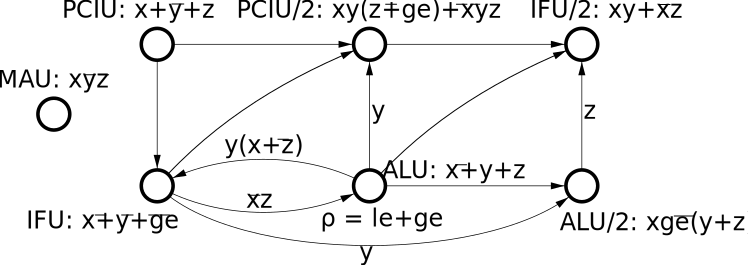
\includegraphics[scale=0.39]{fig/processor_cpog}}\hfill{}\subfloat[Optimal encoding (16 literals)]{

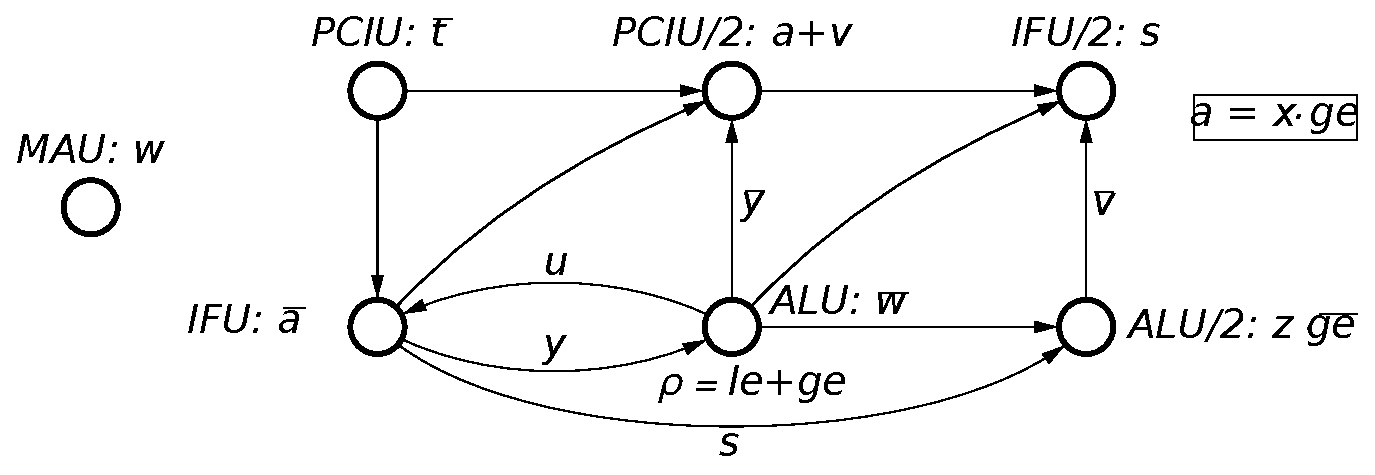
\includegraphics[scale=0.39]{fig/CPOG_L_8}}
\par\end{centering}

\begin{centering}
\subfloat[Optimal encoding $L=3$ (31 literals)]{

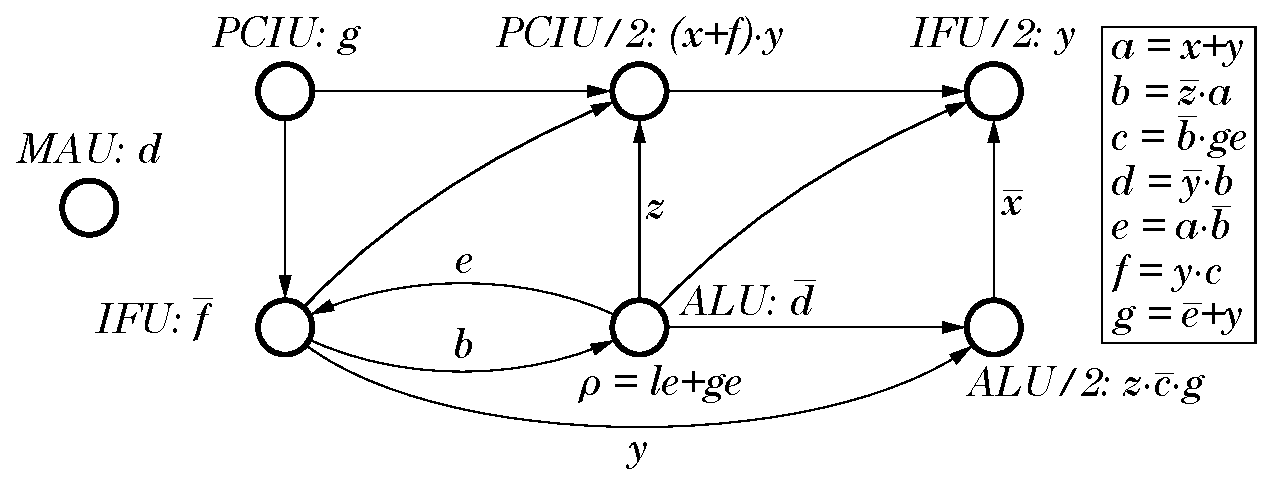
\includegraphics[scale=0.39]{fig/CPOG_L_3}}\hfill{}\subfloat[Optimal encoding $L=5$ (21 literals)]{

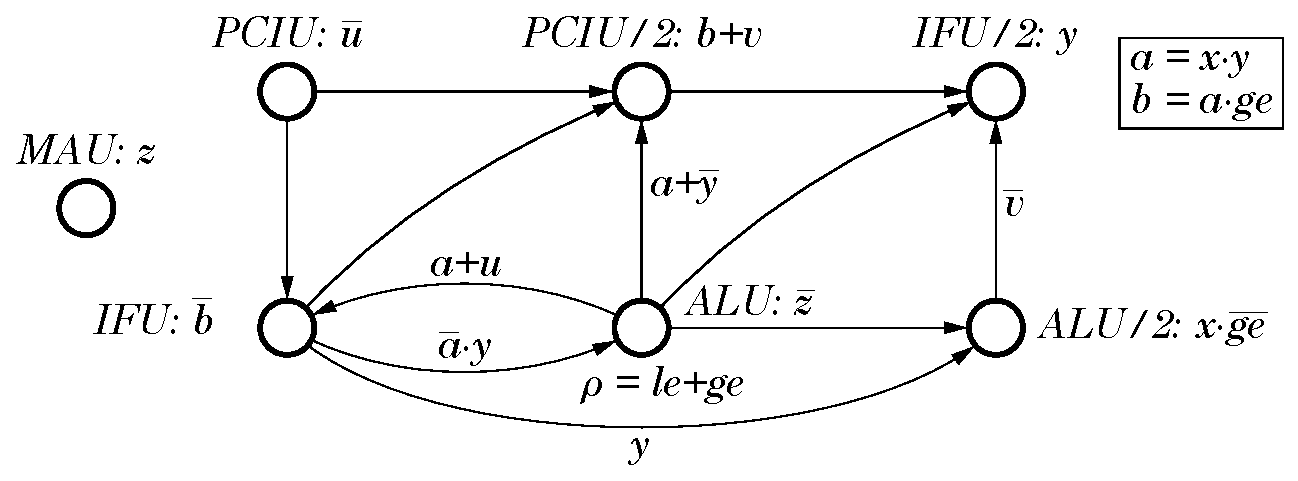
\includegraphics[scale=0.39]{fig/CPOG_L_5}}
\par\end{centering}

\caption{Synthesised CPOGs\label{fig:Synthesised-CPOGs}}
\end{figure}



\subsection{Microcontroller synthesis\label{app-sub-Microcontroller-synthesis}}

Figure~\ref{fig:Synthesised-CPOGs} shows four CPOGs obtained using
instruction encodings shown in Table~\ref{tab:Synthesised-instruction-codes}.
The trivial encoding results in the most complex CPOG shown in Figure~\ref{fig:Synthesised-CPOGs}(a);
it uses three variables $X=\{x,\ y,\ z\}$ and contains 35 literals.
The optimal encoding produces the CPOG with only 16 literals in its
conditions, Figure~\ref{fig:Synthesised-CPOGs}(b), but it uses 8
opcode variables $X=\{x,\ y,\ z,\ u,\ v,\ w,\ s,\ t\}$. Figures~\ref{fig:Synthesised-CPOGs}(c,
d) show the optimal CPOGs encoded with 3 and 5 ($X=\{x,\ y,\ z,\ u,\ v\}$)
variables, respectively; derived variables (denoted by names starting
from $a$) are shown in boxes.

\begin{figure}[h]
\begin{centering}
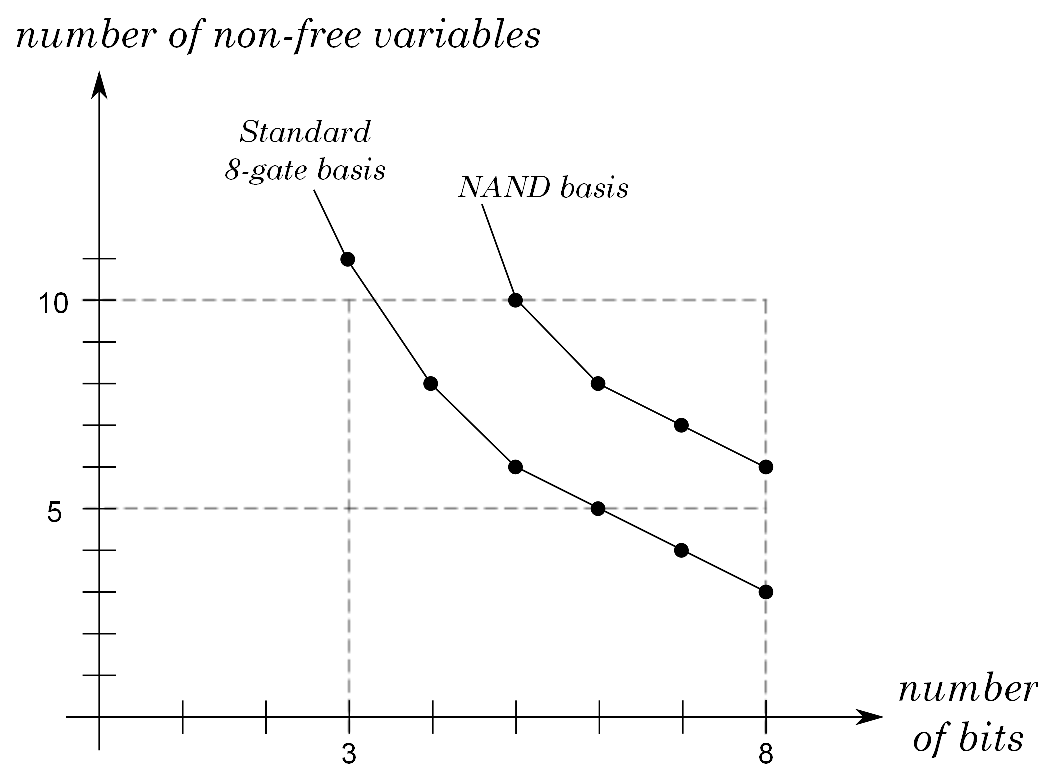
\includegraphics[scale=0.45]{fig/encoding_graph}
\par\end{centering}

\caption{Comparison of different gate bases\label{fig:Comparison-of-different}}
\end{figure}


Figure~\ref{fig:Comparison-of-different} illustrates dependency
of the number of non-free variables on the number of free variables.
As expected, the more free variables we have, the less non-free variables
are needed to satisfy all the encoding constraints. It is interesting
to note that if we restrict our functional basis to NAND gates only
(i.e. if we allow only functions $f_{k}=\overline{f_{i}\cdot f_{j}}$
to be used), the number of non-free variables does not increase dramatically.

Choice of a particular scenario within every CPOG in Figure~\ref{fig:Synthesised-CPOGs}
is highly distributed: every condition is responsible for rendering
only a little portion of the global picture and has a large don't
care set which leads to efficient Boolean minimisation. Note that
flag $le$ turned out to be redundant and was removed from all the
conditions, because original condition $le\cdot\overline{ge}$ is
equivalent to $\overline{ge}$ if the restriction function of ALU
($\rho_{ALU}=le+ge$) is satisfied: $\overline{ge}\cdot(le+ge)\Leftrightarrow le\cdot\overline{ge}$.
Thus it is enough to test only one ALU flag $ge$ to correctly schedule
all the instructions.

\begin{table}[b]
\begin{centering}
\begin{tabular}{|c||c|c|c||c|c|c|}
\hline 
Instructions class & $x$ & $z$ & $v$ & $\phi_{IFU}$ & $\phi_{ALU/2}$ & $\phi_{PCIU/2}$\tabularnewline
\hline 
\hline 
ALU Rn to Rn & 0 & 0 & 0 & 1 & 0 & 0\tabularnewline
\hline 
ALU \#123 to Rn & 0 & 0 & 1 & 1 & 0 & 1\tabularnewline
\hline 
ALU Rn to PC & 0 & 0 & 0 & 1 & 0 & 0\tabularnewline
\hline 
ALU \#123 to PC & 0 & 0 & 0 & 1 & 0 & 0\tabularnewline
\hline 
Memory access & 0 & 0 & 0 & 1 & 0 & 0\tabularnewline
\hline 
Cond. ALU Rn to Rn & 0 & 1 & 0 & 1 & $\overline{ge}$ & 0\tabularnewline
\hline 
Cond. ALU \#123 to Rn & 1 & 1 & 1 & $\overline{ge}$ & $\overline{ge}$ & 1\tabularnewline
\hline 
Cond. ALU \#123 to PC & 1 & 1 & 0 & $\overline{ge}$ & $\overline{ge}$ & $ge$\tabularnewline
\hline 
\hline 
Optimal condition & \multicolumn{3}{c|}{} & $\overline{x\cdot ge}$ & $z\cdot\overline{ge}$ & $x\cdot ge+v$\tabularnewline
\hline 
\end{tabular}
\par\end{centering}

\caption{Encoding of conditions with dynamic variable $ge$\label{app-tab-Encoding-of-non}}
\end{table}


The optimal CPOG (Figure~\ref{fig:Synthesised-CPOGs}(b)) contains
only 16 literals which leads to a twice smaller and faster microcontroller
than the one obtained using the trivial encoding. Note that in this
case it is not possible to reduce the final result to pure 1-restricted
form: the graph contains conditions depending on flag $ge$ which
cannot be mixed with other variables for optimisation purposes as
it is provided by ALU and can be changed during execution of an ALU
operation. Three non 1-restricted conditions are: $\phi(IFU)=\overline{a}=\overline{x\cdot ge}$,
$\phi(ALU/2)=z\cdot\overline{ge}$, and $\phi(PCIU/2)=a+v=x\cdot ge+v$.
It is impossible to use fewer literals for these conditions; this
is clarified in Table~\ref{app-tab-Encoding-of-non}: depending on
the instruction $\phi(IFU)$ has to evaluate either to $1$ or to
$\overline{ge}$ and this choice is delegated to operational variable
$x$ such that $\phi(IFU)=\overline{x\cdot ge}$. Condition $\phi(ALU/2)$
is similar: it must evaluate either to $0$ or to $\overline{ge}$,
hence $\phi(ALU/2)=z\cdot\overline{ge}$. The most complicated case
is presented with condition $\phi(PCIU/2)$ which has three possible
evaluations: $0$, $1$, and $ge$. Two variables are needed to handle
this leading to $\phi(PCIU/2)=x\cdot ge+v$. Optimal encoding of conditions
depending on ALU flags is performed automatically together with all
other conditions as explained in Subsection~\ref{sub:Support-for-dynamic},
thus the optimal result (in terms of the number of used literals)
is guaranteed.

Finally, the chosen CPOG can be mapped into equations to produce the
physical implementation of the microcontroller using the mapping algorithms
from~\cite{2009_mokhov_phd}\cite{2010_mokhov_ieee}.
